\section{RESULTS}
\subsection{CO EMISSION MAPS}

\begin{figure*}[htbp]
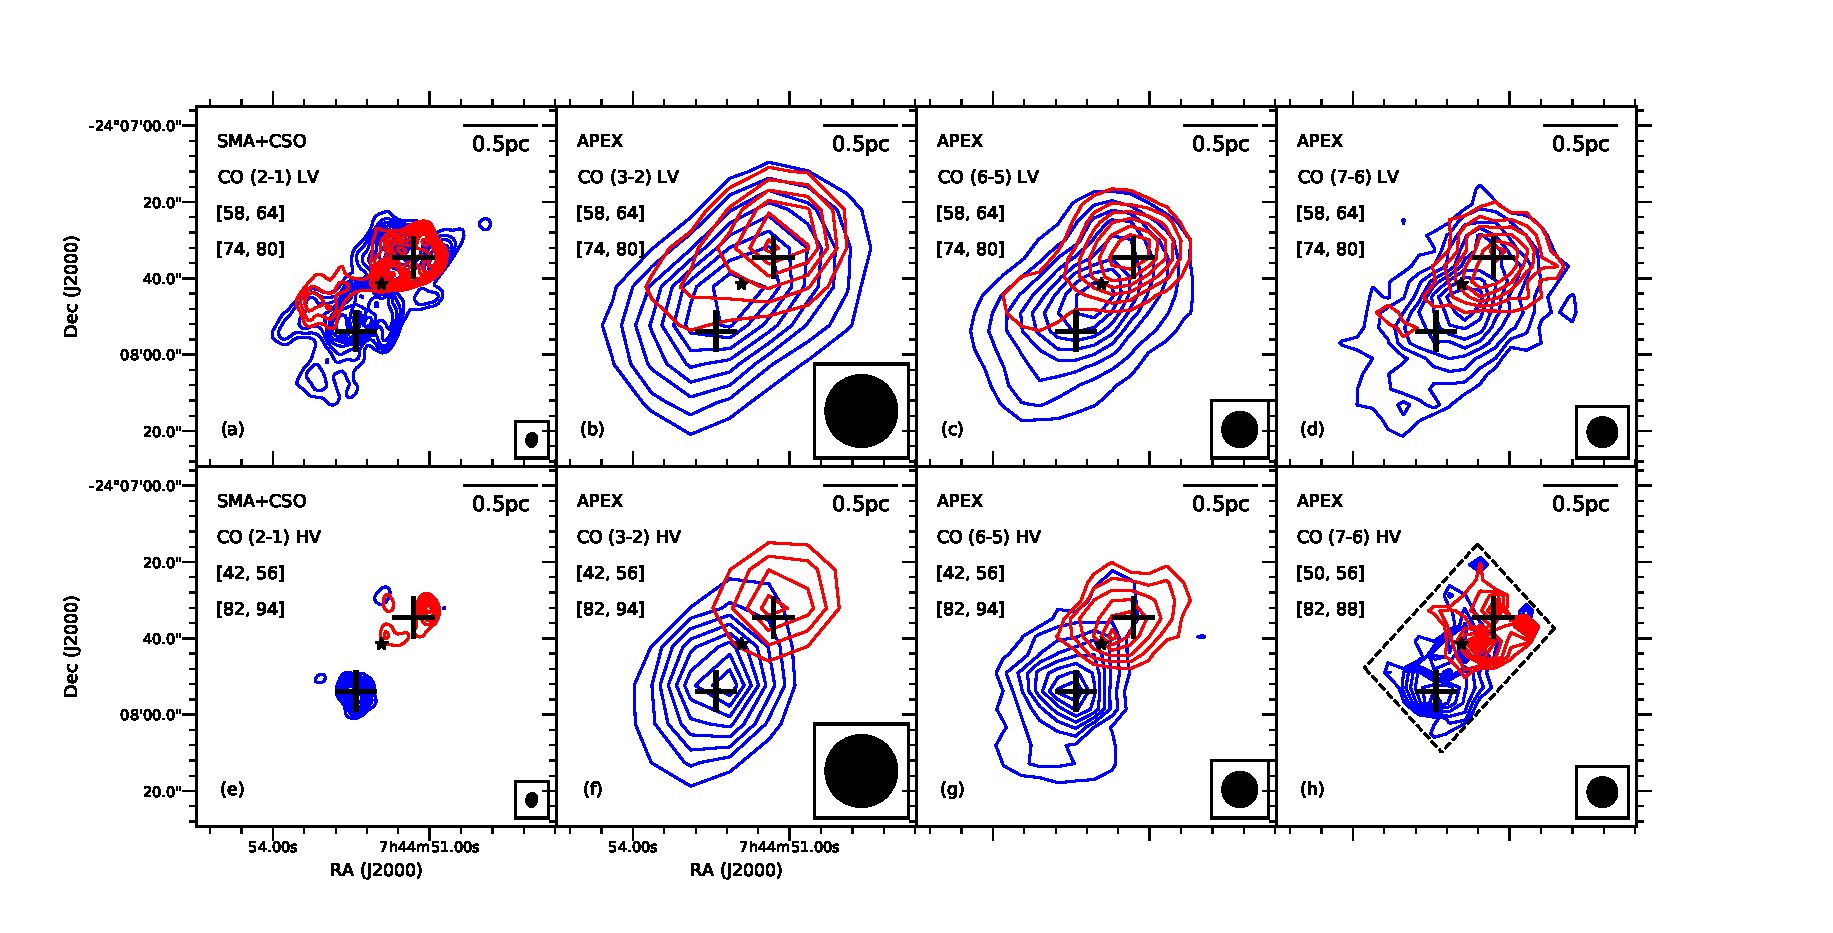
\includegraphics[scale=.65]{./fig/ori_contourall.eps}
\caption{(a)-(d) Low-velocity CO J = (2-1), (3-2), (6-5), (7-6) emissions, integrated from 58 to 64 km s$^{-1} $ for the blueshifted lobe (blue) and from 74 to 80 km s$^{-1}$ for the redshifted lobe (red); (e)-(g) High-velocity CO J = (2-1), (3-2), (6-5) emissions,  integrated from 42 to 56 km s$^{-1} $ for the blueshifted lobe (blue) and from 82 to 94 km s$^{-1}$ for the redshifted lobe (red); (h) High-velocity CO J = (7-6) emission, integrated from 48 to 56 km s$^{-1} $ for the blueshifted lobe (blue) and from 82 to 86 km s$^{-1}$ for the redshifted lobe (red). For (a)-(g), the contour levels start from 20\% and continue at steps of 10\% of the peak emission. For (h), the contour levels start from 30\% and continue at steps of 10\% of the peak emission. Data outside the dashed region are masked out because of the low signal-to-noise ratio. The black star marks the position of a H$_2$O maser spot which is associated with IRAS 07427-2400 \citep{2015PASJ...67...69S}. The beam of each observational dataset is shown in the lower right corner of each panel. \label{fig1}}
\end{figure*}

The cloud velocity ($v_{\mathrm{cloud}}$) with respect to the local standard of rest is $\sim$ 67.5 km s$^{-1}$ \citep{2003A&A...412..175K}. The CO (3-2), (6-5) and (7-6) emissions are detected in velocity ranges from 42 km s$^{-1}$ to 94 km s$^{-1}$, 44 km s$^{-1}$ to 90 km s$^{-1}$, and 48 km s$^{-1}$ to 86 km s$^{-1}$, respectively. Figure \ref{fig1} shows the integrated low-velocity (LV) and high-velocity (HV) emissions of the four transitions. The same velocity ranges with those in \citet{2009ApJ...696...66Q} were chosen to highlight the LV and HV components of the outflowing gas, except for CO (7-6), which we use a smaller velocity range to show the HV emission because of the relatively low signal-to-noise ratio. The outflow morphologies seen in CO (3-2), (6-5) and (7-6) are very similar: a prominent bipolar outflow at (PA) $\sim$ 131${\degr}$ along with a weaker component at PA $\sim$ 101${\degr}$ is detected. The weaker outflow component is only detected at low velocities, while the prominent component is detected at both low and high velocities. Overall, the CO (3-2), (6-5), (7-6) maps presented in Figure \ref{fig1} are very similar to the CO (3-2) map presented by \citet{2003A&A...412..175K}. Due to the limit of angular resolution, the wide-angle structure highlighted by the CO (2-1) emission is not seen in the CO (3-2), (6-5), (7-6) maps.

\subsection{PHYSICAL CONDITIONS OF THE OUTFLOW}
The physical conditions of the outflow could be constrained by comparing the observed line intensities with results of statistical-equilibrium calculations. To study the four lines at the same spatial resolution, we convolved the CO (2-1), (6-5) and (7-6) maps to the same beam size of the CO (3-2) map. The average rms noises are 0.004 K, 0.04 K and 0.10 K for the convolved CO (2-1), (6-5) and (7-6) data, respectively. We then calculated the CO fluxes at (R.A., decl.)$_{J2000}$ = ($07^h44^m52^s.4, -24^d7^m53^s.8$) and (R.A., decl.)$_{J2000}$ = ($07^h44^m51^s.3, -24^d7^m34^s.6$) (marked as two crosses in each panel of Figure \ref{fig1}). The two positions are roughly the peak of the high velocity components of each lobe of the convolved maps of the four transitions. We note that the offsets of the peak positions are within $\sim$ 3$\arcsec$ for different lines at different velocities. To avoid contaminations from the ambient gas, we limited our analyses to velocity ranges of $\le$ 60 km s$^{-1}$ and $\ge$ 74 km s$^{-1}$. And we only focused our analyses on the data with high signal-to-noise ratios in velocities ranges of $\ge$ 48 km s$^{-1}$ and $\le$ 86 km s$^{-1}$. Figure \ref{fig2} shows the observed line wing ratios of main-beam temperatures ($T_{\mathrm{mb}}$) of different CO transitions.  All line ratios in Figure \ref{fig2} are remarkably constant with velocity. Considering that the $^{13}$CO (2-1) emission was only marginally detected in the outflowing gas with high sensitivity observations\citep{2009ApJ...696...66Q}, we assumed the four transitions of $^{12}$CO to be optically thin during the analyses. Both the calibration error and the rms noise were taken into account in the belowing analyses.
%The uncertainty of the observed intensity mainly consists of two parts: the calibration error and the rms noise. At low velocities, the calibration uncertainty dominates the intensity uncertainty, whereas the rms noise is dominant at high velocities. A combination of the rms noise and the calibration error $\sigma_{obs} = (\sigma_{cal}^2 + \sigma_{rms}^2)^{\frac{1}{2}}$ was used as the observational uncertainty in the belowing analyses.
%errors take into account both the rms noise and the calibration uncertainties.

\begin{figure}[tbp]
\plotone{./fig/ratio.eps}
\caption{Ratios of main-beam temperatures of different CO lines at different velocities. Blue symbols denote the measurements from the blueshifted lobe, and red symbols the redshifted lobe. The $V_{\mathrm{outflow}}$ shown here is related to the cloud velocity $v_{\mathrm{cloud}}$ by the relation: $V_{\mathrm{outflow}}$ = $\mid$ $v_{\mathrm{outflow}}$ - $v_{\mathrm{cloud}}\mid$, where $v_{\mathrm{outflow}}$ is the outflow velocity with respect to the local standard of rest. \label{fig2}}
\end{figure}

In a first step, we performed a simple rotation diagram (RD) analysis \citep{1999ApJ...517..209G} to estimate the excitation conditions of the outflowing gas in each velocity interval under the assumption of local thermal equilibrium (LTE). The population of each level is given by 
\begin{equation}
N_{\mathrm{up}} = \frac{N_\mathrm{CO}}{Z} g_\mathrm{up} e^{-E_\mathrm{up}/kT_\mathrm{kin}},
\end{equation}
where $N_\mathrm{up}$ is the column density in the upper state, $g_\mathrm{up}$ the statistical weight of the upper state, $E_\mathrm{up}$ the upper energy level, $k$ the Boltzmann constant, and $Z$ is the partition function.
The rotation diagram for CO at 84 km s$^{-1}$ is shown in Figure \ref{fig3} as an example. Similar rotation diagrams were found at other velocities. It should be noted that the different energy levels in each velocity bin could be well reproduced with a single-component excitation condition, indicating that the four transitions probe the same volume of gas.  

\begin{figure}[tbp]
\plotone{./fig/RD.eps}
\caption{A rotation diagram for CO at 84 km s$^{-1}$.  The fitted line shows the Boltzmann distribution of the rotational populations. The black solid circles show the data with error bars. \label{fig3}}
\end{figure}

In a second step, the non-LTE radiative transfer code RADEX \citep{2007A&A...468..627V} was used to better constrain the gas density ($n_{\mathrm{H}_2}$), the kinetic temperature ($T_{\mathrm{kin}}$) and the CO column density ($N_{\mathrm{CO}}$) of the outflowing gas in each 2 km s$^{-1}$ bin in the Large Velocity Gradient (LVG) approximation. The best fitting results were obtained by minimizing the $\chi^2_{\mathrm{red}}$ between the observed intensities and the model intensities. With four lines observed and three parameters to constrain, our fitting has one degree of freedom. We didn't correct our observed intensities with beam-filling factors. Thus, the derived physical parameters are the average values over the beam.  In Figure \ref{fig:fig4}, the fitting results at 84 km s$^{-1}$ are shown as examples of the $\chi^2_{\mathrm{red}}$ distribution. Similar $\chi^2_{\mathrm{red}}$ distribution profiles were found at other velocities. The $\chi^2_{\mathrm{red}}$ has only one minimum in [$T$, $N$] planes. The $\chi^2_{\mathrm{red}}$ distribution in the [$T$, $n$] and [$n$, $N$] planes show that the gas is thermalized and no upper limits to the density could be derived, which confirms the LTE assumption used in the rotation diagram analysis. The $\chi^2_{\mathrm{red}}$ of the best fitting results varies from 0.10 to 1.72 at different velocities. Though the best-fitted $\chi^2_{\mathrm{red}}$ have different values at different velocities, the $\chi^2_{\mathrm{red}}$ distributions show similarity in morphology, indicating that the uncertainties of the fitted parameters may have similar level at different velocities. So we derive the uncertainties of each parameter of the LVG analysis from the 1$\sigma$ confidence region in the $N$-$T$-$n$ 3-dimensional space at the velocities where $\chi^2_{\mathrm{red}} \sim 1$ as the representative uncertainties of the fitted parameters. The 1$\sigma$ confidence ranges of temperatures are about 40 K - 60 K. The lower limits of gas densities ($n_{\mathrm{lower}}$) are around 10$^5$ cm$^{-3}$, larger than the critical densities of the four lines. The uncertainties of CO column densities are $\sim$ 10 \%. The modeling results predict that the four transitions are optically thin in the outflowing gas, which is consistent with our assumptions. Figure \ref{fig:figa1} shows the comparison of the observed CO intensities with the LVG modeling results in each velocity bin. 

\begin{figure*}
\gridline{\fig{./fig/chiimage_nco_paper.eps}{0.5\textwidth}{(a)}
        \fig{./fig/chiimage_nh2_paper.eps}{0.5\textwidth}{(b)}}
 \gridline{\fig{./fig/chiimage_tkin_paper.eps}{0.5\textwidth}{(c)}
      \fig{./fig/chiimage_nh2_low_paper.eps}{0.5\textwidth}{(d)}}
\caption{(a)-(c) The $\chi^2_{\mathrm{red}}$ distribution at 84 km s$^{-1}$ in the [$T$, $n$], [$T$, $N$] and [$n$, $N$] planes, with all other parameters fixed to the values of the best fitting results at this velocity; (d) The $\chi^2_{\mathrm{red}}$ distribution at 84 km s$^{-1}$ in the [$T$, $N$] plane, with the density fixed to the lower limit of density in the 1$\sigma$ confidence region of the fitting result at this velocity. The $\chi^2_{\mathrm{red}}$ of the best fitting result is $\sim$1.00 at 84 km s$^{-1}$. The Solid white contours show the 1$\sigma$ confidence levels. \label{fig:fig4}}
\end{figure*}

Figure \ref{fig:fig5} shows the outflowing gas temperature and the CO column density as functions of gas velocity, estimated from the rotation diagram analysis and the LVG analysiss. The $N$-$V$ diagram shows a clear decreasing trend of CO column density with outflow velocity, while the $T$-$V$ diagram shows that the gas temperature has no obvious dependence on gas velocity. The best fitted $\chi^2_{\mathrm{red}}$ at different velocities calculated from the LVG analysis are shown in the $N$-$V$ diagram. 

\begin{figure*}
\gridline{\fig{./fig/tv_paper.eps}{0.5\textwidth}{(a)}
          \fig{./fig/Nv_paper.eps}{0.5\textwidth}{(b)}
          }
\caption{$T$-$V$ and $N$-$V$ diagrams of the G240 outflow, estimated from the rotation diagram analysis (blue x marker for blue lobe and red x marker for red lobe) and the LVG analyses (blue open squares for blue lobe and red open squares for red lobe). The best fitted $\chi^2_{\mathrm{red}}$ calculated from the LVG analysis are shown in the $N$-$V$ diagram. \label{fig:fig5}}
\end{figure*}

We then performed the rotation diagram analysis and the LVG analysis again with the line intensities calculated from several different positions and got similar results with previous analysis. Thus, we exclude the systematic bias from the choice of positions for measuring the line intensities.
